\documentclass{article}
\usepackage{paralist}
\usepackage{graphicx}
\usepackage{fancyhdr}
\usepackage{datetime}


\begin{document}

\title{Interactive Graphics Report\\
		Homework 1}
\author{Jean-Pierre Richa}
\date{May 2018}
\maketitle
\section {Introduction}
\textbf {In this report, we are going to explain the work done for the interactive graphics second homework.
The homework contained 3 questions, which we are going to see and explain their implementation in details.}

\section {Implementation}
\textbf{In this section, we are going to address each problem and discuss its implementation. The code pieces will not be shown in the report, because it is scattered in multiple files. All of the code is already commented using the question number it belongs to.}


\begin{enumerate}
\item \textbf{Create a Hierarchical model of a dog}:

In this question we were supposed to create a hierarchical structure of a simplified dog using cubes. The hierarchical structure is obtained through creating nodes in a hierarchical way where each node has a sibling and a child. The child is usually the node following the current one, and the sibling is the node parallel or next to the current node. The whole structure(dog) have to be aligned along the X axis, because as we will see in the 3rd question, we need to make the dog walk along the X axis. First of all, and in order to have a clean implementation, we need to start by the body of the dog and the head, because since this is a hierarchical structure, and all of the other nodes in this implementation are created with respect to the body of the dog, it can be seen in the JS file in the initNodes function that we are translating the other parts using the body width and height. So after creating all the nodes specifying if it is a sibling or a child of another node, and specifying the location of the node using the body of the dog as reference, we will obtain all the parts connected to each other, but in order to obtain the final dog shape, we need to adjust the angles of the tail, legs, and head to better visualise it. Figure1 in in the end of the report gives a clearer idea about the structure.

\item \textbf{Add a checkerboard pattern texture}:

Here we had to add a checkerboard texture with a linear decrease of intensity from the front to the back of the body. It is important to understand that is order to obtain this kind of textures, we have to use 2 different images having 2 different textures, because they will be created one on top of the other, which results with the checkerboard pattern. as for the intensity of the texture, it can be obtained through iterating through the body parts of the dog and decreasing the colors intensity "linearly" untill we reach the full black color as shown on the different body parts. To better visualise what I talked about above, a picture (Figure 2) is provided in the end of the report.


\item \textbf{Add a button to make the dog walk}:

The goal from this question was to add a button that when pressed, the dog should start walking from an initial position (which i chose here the left side of the canvas, and while walking the dog should change its position until it reaches the right side of the screen, which is the final position. here i added a condition which makes the dog walks back and forth while changing orientation that corresponds to the walking direction(if it is walking to the right, then the dog will be oriented to the right). Here also, we had to make the head move and keep looking to the position of the viewer, which in this case is us, so the dog will start with a specific head orientation, and will start changing it while walking to keep looking at the viewer. A very important point here is that while the dog is standing still, we should only see 2 legs(front leg and rear leg), because front-left and front-right legs should be aligned, as well as rear-left and rear-right, so the upper legs and the lower legs should have the same initial angles. When the legs will be moving, we should see the right legs(front and rear) moving in the same way through increasing the angle of rotation of the "right" upper and lower legs simultaneously (front and rear), same for the left legs(front and rear), but right legs should move in the opposite direction of the left legs, so we can obtain natural walking. Since the dog is translating along the X axis, the tail and legs are rotating around the Z axis, and the head is rotating around the Z and the Y axis also, because I wanted to show a more natural movement. What i did here to obtain as much natural walk as possible, is that I increased the position along the X axis after each complete movement  of 1 side of the legs.



\section {Conclusion}
\textbf{It was really interesting working with hierarchical structure, because here for example we had to focus only on the body when moving the dog, and not on the whole body parts, which makes it easier to implement more complex objects especially if we have an object with more dependent parts. Below, 2 photos are shown, which explain the hierarchical structure of the dog's body parts, and a photo of the dog while standing where the checkerboard pattern structure is also clear.}







\begin{figure}[!ht]
\centering
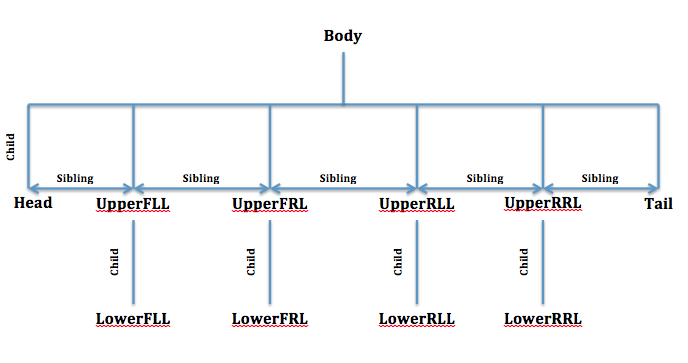
\includegraphics[scale=0.50]{HW1}
\caption{Dog Hierarchical Structure}
\label{fig:fig1}
\end{figure}

\begin{figure}[!ht]
\centering
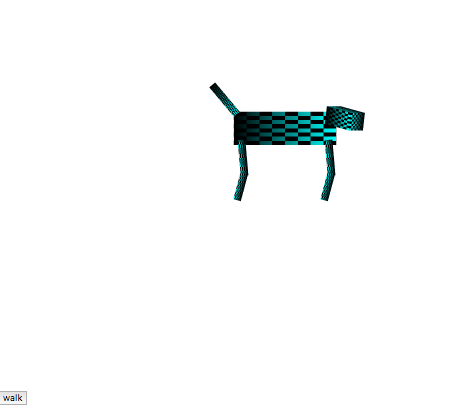
\includegraphics[scale=0.50]{HW2}
\caption{Final Result}
\label{fig:fig1}
\end{figure}




\end{enumerate}
\end{document}